% Created by tikzDevice version 0.8.1 on 2015-06-28 21:11:30
% !TEX encoding = UTF-8 Unicode
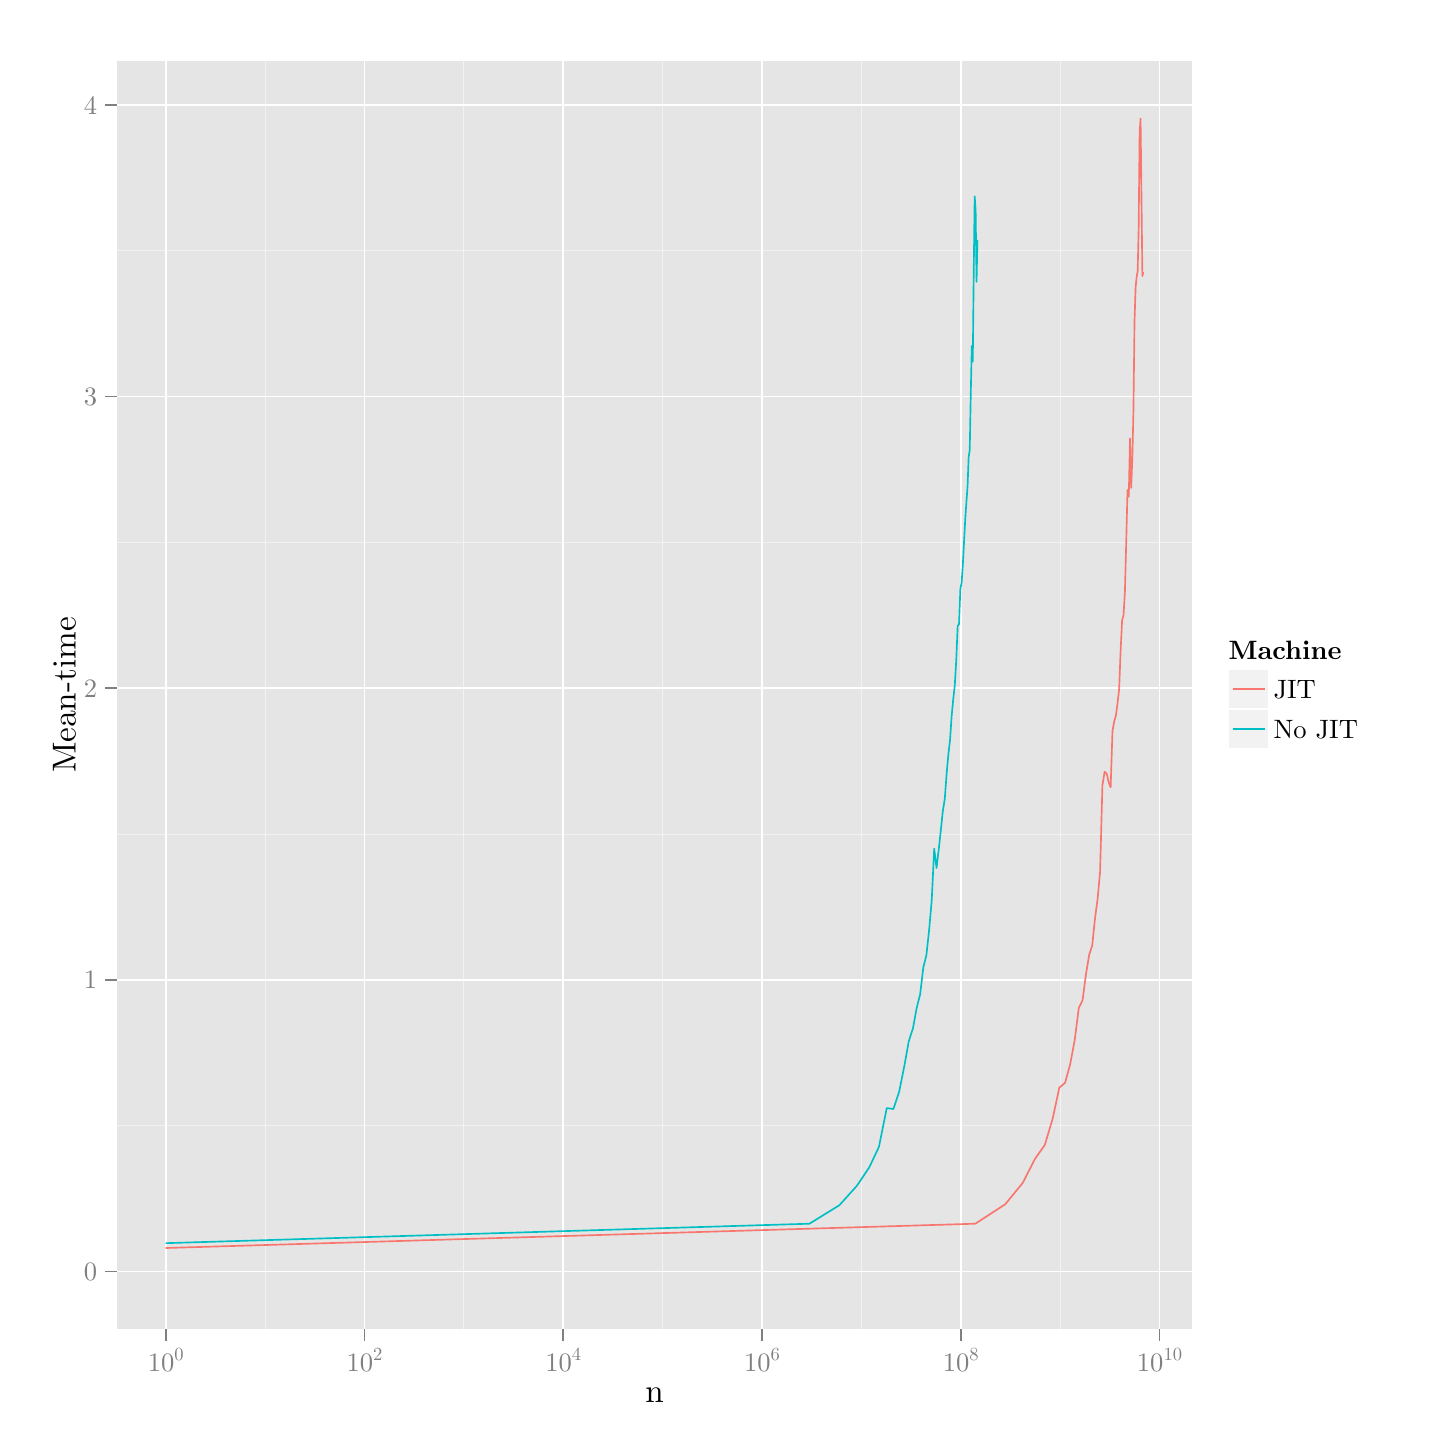
\begin{tikzpicture}[x=1pt,y=1pt]
\definecolor{fillColor}{RGB}{255,255,255}
\path[use as bounding box,fill=fillColor,fill opacity=0.00] (0,0) rectangle (505.89,505.89);
\begin{scope}
\path[clip] (  0.00,  0.00) rectangle (505.89,505.89);
\definecolor{drawColor}{RGB}{255,255,255}
\definecolor{fillColor}{RGB}{255,255,255}

\path[draw=drawColor,line width= 0.6pt,line join=round,line cap=round,fill=fillColor] (  0.00,  0.00) rectangle (505.89,505.89);
\end{scope}
\begin{scope}
\path[clip] ( 32.22, 35.66) rectangle (420.79,493.85);
\definecolor{fillColor}{gray}{0.90}

\path[fill=fillColor] ( 32.22, 35.66) rectangle (420.79,493.85);
\definecolor{drawColor}{gray}{0.95}

\path[draw=drawColor,line width= 0.3pt,line join=round] ( 32.22,109.17) --
	(420.79,109.17);

\path[draw=drawColor,line width= 0.3pt,line join=round] ( 32.22,214.53) --
	(420.79,214.53);

\path[draw=drawColor,line width= 0.3pt,line join=round] ( 32.22,319.89) --
	(420.79,319.89);

\path[draw=drawColor,line width= 0.3pt,line join=round] ( 32.22,425.25) --
	(420.79,425.25);

\path[draw=drawColor,line width= 0.3pt,line join=round] ( 85.80, 35.66) --
	( 85.80,493.85);

\path[draw=drawColor,line width= 0.3pt,line join=round] (157.62, 35.66) --
	(157.62,493.85);

\path[draw=drawColor,line width= 0.3pt,line join=round] (229.44, 35.66) --
	(229.44,493.85);

\path[draw=drawColor,line width= 0.3pt,line join=round] (301.27, 35.66) --
	(301.27,493.85);

\path[draw=drawColor,line width= 0.3pt,line join=round] (373.09, 35.66) --
	(373.09,493.85);
\definecolor{drawColor}{RGB}{255,255,255}

\path[draw=drawColor,line width= 0.6pt,line join=round] ( 32.22, 56.49) --
	(420.79, 56.49);

\path[draw=drawColor,line width= 0.6pt,line join=round] ( 32.22,161.85) --
	(420.79,161.85);

\path[draw=drawColor,line width= 0.6pt,line join=round] ( 32.22,267.21) --
	(420.79,267.21);

\path[draw=drawColor,line width= 0.6pt,line join=round] ( 32.22,372.57) --
	(420.79,372.57);

\path[draw=drawColor,line width= 0.6pt,line join=round] ( 32.22,477.94) --
	(420.79,477.94);

\path[draw=drawColor,line width= 0.6pt,line join=round] ( 49.88, 35.66) --
	( 49.88,493.85);

\path[draw=drawColor,line width= 0.6pt,line join=round] (121.71, 35.66) --
	(121.71,493.85);

\path[draw=drawColor,line width= 0.6pt,line join=round] (193.53, 35.66) --
	(193.53,493.85);

\path[draw=drawColor,line width= 0.6pt,line join=round] (265.36, 35.66) --
	(265.36,493.85);

\path[draw=drawColor,line width= 0.6pt,line join=round] (337.18, 35.66) --
	(337.18,493.85);

\path[draw=drawColor,line width= 0.6pt,line join=round] (409.00, 35.66) --
	(409.00,493.85);
\definecolor{drawColor}{RGB}{248,118,109}

\path[draw=drawColor,line width= 0.6pt,line join=round] ( 49.88, 64.92) --
	(342.43, 73.70) --
	(353.24, 80.72) --
	(359.56, 88.45) --
	(364.05, 97.23) --
	(367.53,102.14) --
	(370.37,111.63) --
	(372.78,122.86) --
	(374.86,124.62) --
	(376.70,131.29) --
	(378.34,140.07) --
	(379.82,151.66) --
	(381.18,154.47) --
	(382.43,163.96) --
	(383.59,170.98) --
	(384.66,174.14) --
	(385.67,183.97) --
	(386.61,191.00) --
	(387.51,200.83) --
	(388.35,232.09) --
	(389.15,237.01) --
	(389.91,236.30) --
	(390.64,233.14) --
	(391.33,231.39) --
	(391.99,251.76) --
	(392.63,255.27) --
	(393.24,257.38) --
	(393.83,261.94) --
	(394.40,266.86) --
	(394.94,280.91) --
	(395.47,291.80) --
	(395.98,293.55) --
	(396.48,301.98) --
	(396.96,320.24) --
	(397.42,338.86) --
	(397.88,336.40) --
	(398.32,357.47) --
	(398.74,339.56) --
	(399.16,350.10) --
	(399.56,367.30) --
	(399.96,399.97) --
	(400.34,411.91) --
	(400.72,415.77) --
	(401.09,417.88) --
	(401.45,433.33) --
	(401.80,468.10) --
	(402.14,473.02) --
	(402.47,444.57) --
	(402.80,416.12) --
	(403.12,417.53);
\definecolor{drawColor}{RGB}{0,191,196}

\path[draw=drawColor,line width= 0.6pt,line join=round] ( 49.88, 66.67) --
	(282.49, 73.70) --
	(293.30, 80.37) --
	(299.62, 87.39) --
	(304.11, 94.07) --
	(307.59,101.44) --
	(310.43,115.49) --
	(312.84,115.14) --
	(314.92,121.46) --
	(316.76,130.59) --
	(318.40,139.72) --
	(319.89,144.29) --
	(321.24,151.66) --
	(322.49,156.58) --
	(323.65,166.41) --
	(324.73,170.63) --
	(325.73,179.76) --
	(326.68,190.65) --
	(327.57,209.26) --
	(328.41,202.24) --
	(329.21,208.91) --
	(329.97,215.93) --
	(330.70,222.96) --
	(331.39,227.17) --
	(332.06,236.30) --
	(332.69,243.33) --
	(333.30,248.60) --
	(333.89,257.38) --
	(334.46,263.35) --
	(335.01,268.26) --
	(335.54,277.40) --
	(336.05,289.69) --
	(336.54,290.39) --
	(337.02,303.03) --
	(337.49,305.49) --
	(337.94,312.17) --
	(338.38,320.59) --
	(338.81,328.67) --
	(339.22,334.64) --
	(339.63,340.26) --
	(340.02,350.80) --
	(340.41,353.26) --
	(340.78,373.28) --
	(341.15,390.84) --
	(341.51,385.22) --
	(341.86,418.23) --
	(342.20,444.92) --
	(342.54,440.00) --
	(342.87,414.02) --
	(343.19,429.12);
\end{scope}
\begin{scope}
\path[clip] (  0.00,  0.00) rectangle (505.89,505.89);
\definecolor{drawColor}{gray}{0.50}

\node[text=drawColor,anchor=base east,inner sep=0pt, outer sep=0pt, scale=  0.96] at ( 25.11, 53.18) {0};

\node[text=drawColor,anchor=base east,inner sep=0pt, outer sep=0pt, scale=  0.96] at ( 25.11,158.54) {1};

\node[text=drawColor,anchor=base east,inner sep=0pt, outer sep=0pt, scale=  0.96] at ( 25.11,263.90) {2};

\node[text=drawColor,anchor=base east,inner sep=0pt, outer sep=0pt, scale=  0.96] at ( 25.11,369.27) {3};

\node[text=drawColor,anchor=base east,inner sep=0pt, outer sep=0pt, scale=  0.96] at ( 25.11,474.63) {4};
\end{scope}
\begin{scope}
\path[clip] (  0.00,  0.00) rectangle (505.89,505.89);
\definecolor{drawColor}{gray}{0.50}

\path[draw=drawColor,line width= 0.6pt,line join=round] ( 27.95, 56.49) --
	( 32.22, 56.49);

\path[draw=drawColor,line width= 0.6pt,line join=round] ( 27.95,161.85) --
	( 32.22,161.85);

\path[draw=drawColor,line width= 0.6pt,line join=round] ( 27.95,267.21) --
	( 32.22,267.21);

\path[draw=drawColor,line width= 0.6pt,line join=round] ( 27.95,372.57) --
	( 32.22,372.57);

\path[draw=drawColor,line width= 0.6pt,line join=round] ( 27.95,477.94) --
	( 32.22,477.94);
\end{scope}
\begin{scope}
\path[clip] (  0.00,  0.00) rectangle (505.89,505.89);
\definecolor{drawColor}{gray}{0.50}

\path[draw=drawColor,line width= 0.6pt,line join=round] ( 49.88, 31.39) --
	( 49.88, 35.66);

\path[draw=drawColor,line width= 0.6pt,line join=round] (121.71, 31.39) --
	(121.71, 35.66);

\path[draw=drawColor,line width= 0.6pt,line join=round] (193.53, 31.39) --
	(193.53, 35.66);

\path[draw=drawColor,line width= 0.6pt,line join=round] (265.36, 31.39) --
	(265.36, 35.66);

\path[draw=drawColor,line width= 0.6pt,line join=round] (337.18, 31.39) --
	(337.18, 35.66);

\path[draw=drawColor,line width= 0.6pt,line join=round] (409.00, 31.39) --
	(409.00, 35.66);
\end{scope}
\begin{scope}
\path[clip] (  0.00,  0.00) rectangle (505.89,505.89);
\definecolor{drawColor}{gray}{0.50}

\node[text=drawColor,anchor=base west,inner sep=0pt, outer sep=0pt, scale=  0.96] at ( 43.41, 20.31) {10};

\node[text=drawColor,anchor=base west,inner sep=0pt, outer sep=0pt, scale=  0.67] at ( 53.00, 24.24) {0};

\node[text=drawColor,anchor=base west,inner sep=0pt, outer sep=0pt, scale=  0.96] at (115.23, 20.31) {10};

\node[text=drawColor,anchor=base west,inner sep=0pt, outer sep=0pt, scale=  0.67] at (124.83, 24.24) {2};

\node[text=drawColor,anchor=base west,inner sep=0pt, outer sep=0pt, scale=  0.96] at (187.05, 20.31) {10};

\node[text=drawColor,anchor=base west,inner sep=0pt, outer sep=0pt, scale=  0.67] at (196.65, 24.24) {4};

\node[text=drawColor,anchor=base west,inner sep=0pt, outer sep=0pt, scale=  0.96] at (258.88, 20.31) {10};

\node[text=drawColor,anchor=base west,inner sep=0pt, outer sep=0pt, scale=  0.67] at (268.47, 24.24) {6};

\node[text=drawColor,anchor=base west,inner sep=0pt, outer sep=0pt, scale=  0.96] at (330.70, 20.31) {10};

\node[text=drawColor,anchor=base west,inner sep=0pt, outer sep=0pt, scale=  0.67] at (340.30, 24.24) {8};

\node[text=drawColor,anchor=base west,inner sep=0pt, outer sep=0pt, scale=  0.96] at (400.84, 20.31) {10};

\node[text=drawColor,anchor=base west,inner sep=0pt, outer sep=0pt, scale=  0.67] at (410.44, 24.24) {1};

\node[text=drawColor,anchor=base west,inner sep=0pt, outer sep=0pt, scale=  0.67] at (413.80, 24.24) {0};
\end{scope}
\begin{scope}
\path[clip] (  0.00,  0.00) rectangle (505.89,505.89);
\definecolor{drawColor}{RGB}{0,0,0}

\node[text=drawColor,anchor=base,inner sep=0pt, outer sep=0pt, scale=  1.20] at (226.50,  9.03) {n};
\end{scope}
\begin{scope}
\path[clip] (  0.00,  0.00) rectangle (505.89,505.89);
\definecolor{drawColor}{RGB}{0,0,0}

\node[text=drawColor,rotate= 90.00,anchor=base,inner sep=0pt, outer sep=0pt, scale=  1.20] at ( 17.30,264.75) {Mean-time};
\end{scope}
\begin{scope}
\path[clip] (  0.00,  0.00) rectangle (505.89,505.89);
\definecolor{fillColor}{RGB}{255,255,255}

\path[fill=fillColor] (429.65,240.91) rectangle (484.98,288.59);
\end{scope}
\begin{scope}
\path[clip] (  0.00,  0.00) rectangle (505.89,505.89);
\definecolor{drawColor}{RGB}{0,0,0}

\node[text=drawColor,anchor=base west,inner sep=0pt, outer sep=0pt, scale=  0.96] at (433.92,277.70) {\bfseries Machine};
\end{scope}
\begin{scope}
\path[clip] (  0.00,  0.00) rectangle (505.89,505.89);
\definecolor{drawColor}{RGB}{255,255,255}
\definecolor{fillColor}{gray}{0.95}

\path[draw=drawColor,line width= 0.6pt,line join=round,line cap=round,fill=fillColor] (433.92,259.63) rectangle (448.38,274.09);
\end{scope}
\begin{scope}
\path[clip] (  0.00,  0.00) rectangle (505.89,505.89);
\definecolor{drawColor}{RGB}{248,118,109}

\path[draw=drawColor,line width= 0.6pt,line join=round] (435.37,266.86) -- (446.93,266.86);
\end{scope}
\begin{scope}
\path[clip] (  0.00,  0.00) rectangle (505.89,505.89);
\definecolor{drawColor}{RGB}{255,255,255}
\definecolor{fillColor}{gray}{0.95}

\path[draw=drawColor,line width= 0.6pt,line join=round,line cap=round,fill=fillColor] (433.92,245.18) rectangle (448.38,259.63);
\end{scope}
\begin{scope}
\path[clip] (  0.00,  0.00) rectangle (505.89,505.89);
\definecolor{drawColor}{RGB}{0,191,196}

\path[draw=drawColor,line width= 0.6pt,line join=round] (435.37,252.41) -- (446.93,252.41);
\end{scope}
\begin{scope}
\path[clip] (  0.00,  0.00) rectangle (505.89,505.89);
\definecolor{drawColor}{RGB}{0,0,0}

\node[text=drawColor,anchor=base west,inner sep=0pt, outer sep=0pt, scale=  0.96] at (450.18,263.55) {JIT};
\end{scope}
\begin{scope}
\path[clip] (  0.00,  0.00) rectangle (505.89,505.89);
\definecolor{drawColor}{RGB}{0,0,0}

\node[text=drawColor,anchor=base west,inner sep=0pt, outer sep=0pt, scale=  0.96] at (450.18,249.10) {No JIT};
\end{scope}
\end{tikzpicture}
